% =========================================================================
% Veritas: Version-Aware Enterprise Policy Intelligence
% IEEE Journal Manuscript — Camera-Ready Publication Source
% Author: Suyash Pradhan
% Frozen Application Commit: 61d64b71c298c3c505f2eeeef3c94829dfb55f75
% Characterization Harness Commit: 449e69b343dd8c3483120ea7b00bf193ea25df15
% Master Random Seed: SEED=42
% =========================================================================
\documentclass[journal]{IEEEtran}

\usepackage{cite}
\usepackage{amsmath,amssymb,amsfonts}
\usepackage{algorithm}
\usepackage{algorithmic}
\usepackage{graphicx}
\usepackage{booktabs}
\usepackage{multirow}
\usepackage{array}
\usepackage{tabularx}
\usepackage{url}
\usepackage{microtype}
\usepackage{textcomp}
\usepackage{balance}

% ----- Macros -----
\newcommand{\sys}{Veritas}
\newcommand{\ms}{\,\mathrm{ms}}
\newcolumntype{Y}{>{\centering\arraybackslash}X}
\newcolumntype{Z}{>{\raggedright\arraybackslash}X}
\newcommand{\D}{\mathbb{D}}

\setlength{\textfloatsep}{3pt plus 1pt minus 1pt}
\setlength{\floatsep}{3pt plus 1pt minus 1pt}
\setlength{\intextsep}{3pt plus 1pt minus 1pt}
\setlength{\dbltextfloatsep}{3pt plus 1pt minus 1pt}
\setlength{\dblfloatsep}{3pt plus 1pt minus 1pt}
\setlength{\abovecaptionskip}{2pt plus 1pt minus 1pt}
\setlength{\belowcaptionskip}{1pt plus 1pt minus 1pt}
\setlength{\abovedisplayskip}{2.5pt plus 1pt minus 1pt}
\setlength{\belowdisplayskip}{2.5pt plus 1pt minus 1pt}
\setlength{\abovedisplayshortskip}{1pt plus 1pt}
\setlength{\belowdisplayshortskip}{1pt plus 1pt}

\begin{document}

\title{\sys{}: Version-Aware Enterprise Policy Intelligence via
Incremental Knowledge Compilation and Adaptive Multi-Tier Retrieval}

\author{Suyash~Pradhan%
\thanks{S. Pradhan is with the Department of Computer Science and Engineering
(e-mail: suyashpradhan06@gmail.com).}}

\markboth{IEEE Transactions / Journal Manuscript}{\sys{}: Version-Aware Enterprise Policy Intelligence}

\maketitle

% =========================================================================
\begin{abstract}
Enterprise policy repositories undergo continuous revision, requiring historical and active provisions to coexist under strict role-based access. Conventional retrieval-augmented generation (RAG) models rank evidence primarily by semantic similarity, risking temporal version inversion, full re-indexing overhead, generative latency on deterministic lookups, and authorization leakage. We present \sys{}, an enterprise policy intelligence system that treats retrieval as a constrained systems problem: a composite eligibility predicate $E(c,u,t_q)=V(c,t_q)\cdot A(c,u)$ enforces date-bounded validity and role authorization prior to evidence admission and reranking. \sys{} integrates a seven-stage SHA-256 incremental compiler, an adaptive four-tier query router, and a calibrated NLI verification layer. Across an audited evaluation framework spanning a 301-query baseline and an expanded 922-query characterization suite (120 policies, ~3,000 chunks, 32 user archetypes), \sys{} achieved zero observed unauthorized evidence leakage across 3,840 evaluations (95\% upper bound $<0.08\%$) and $94.47\%$ top-1 chunk retrieval recall via hybrid RRF and cross-encoder reranking. Deterministic and refusal paths resolved $63.4\%$ of queries ($4.50\ms$ system median latency). On a 5\% amendment delta over 3,000 chunks, the incremental compiler avoided $95.0\%$ of re-embeddings ($24.95\times$ speedup, $2.10\text{s}$ vs.\ $52.4\text{s}$ rebuild). Isotonic regression achieved $0.041$ validation ECE, while runtime ECE reached $0.2954$ under distribution shift. These results demonstrate that pre-retrieval constraint enforcement provides verifiable data isolation and latency reduction for enterprise policy QA.
\end{abstract}

\begin{IEEEkeywords}
Retrieval-augmented generation, temporal information retrieval, version-aware retrieval, incremental indexing, enterprise knowledge management, adaptive query routing, confidence calibration, natural language inference.
\end{IEEEkeywords}

% =========================================================================
\section{Introduction}
\IEEEPARstart{E}{nterprise} governance, corporate administration, information security, and regulatory compliance depend on policy documents that undergo continuous revision. Corporate travel allowances, parental leave provisions, remote-work rules, and security controls each undergo periodic amendment, requiring retrieval mechanisms that distinguish historical validity from current applicability while respecting authorization boundaries.

Conventional retrieval-augmented generation (RAG) architectures rank semantic similarity over document collections \cite{lewis2020rag,gao2024rag_survey}. Within enterprise policy repositories, four operational risks are prominent:
\textbf{(1) Temporal version inversion:} superseded clauses are retrieved for current queries, or obsolete provisions are returned for historical inquiries \cite{campos2014temporal,huwiler2025versionrag,timelyrag2026};
\textbf{(2) Re-indexing overhead:} document amendments trigger corpus-wide re-embedding;
\textbf{(3) Generative latency:} deterministic policy facts incur unnecessary autoregressive inference;
\textbf{(4) Scope leakage:} unpartitioned retrieval exposes confidential information across roles \cite{almasoud2026sdrag,mu2026securerag}.

This paper investigates: \textit{Can an enterprise policy retrieval architecture simultaneously enforce date-bounded temporal validity and role-based authorization constraints while reducing unnecessary generation latency and incremental compilation overhead, without degrading retrieval accuracy on legitimate requests?}

To answer this question, \sys{} treats policy retrieval as a constrained systems problem. While individual components such as dense embeddings, lexical indexes, cross-encoders, and NLI classifiers exist in isolation, \sys{} formulates temporal validity intervals, role authorization, cryptographic delta compilation, and tiered routing as an integrated architecture where constraints are evaluated before candidate evidence enters reranking or generative prompt assembly.

The technical contributions of this work comprise:
\begin{enumerate}\setlength{\itemsep}{0pt}\setlength{\parsep}{0pt}\setlength{\topsep}{1pt}
  \item \textbf{Composite eligibility predicate:} closed date-bounded validity intervals and role-derived authorization enforced at every pipeline tier before evidence admission and reranking.
  \item \textbf{Seven-stage incremental compiler:} SHA-256 chunk hashing, delta partitioning, targeted embedding, and dynamic vector overlays, reducing dominant embedding complexity from $O(N\cdot d)$ to $O(|\Delta|\cdot d)$.
  \item \textbf{Adaptive four-tier router:} fact resolution (Tier~0), canonical QA matching (Tier~1), hybrid dense-sparse retrieval (Tier~2), and structural version diffing (Tier~3), resolving deterministic traffic without generative LLM overhead.
  \item \textbf{Security and evidence controls:} pre-reranking scope gating, NLI entailment verification, post-hoc calibrated confidence, safe abstention, and tamper-evident audit traceability.
  \item \textbf{Empirical characterization:} multi-dimensional evaluation demonstrating zero observed leakage across 3,840 authorization decisions, $94.47\%$ top-1 chunk retrieval recall, a $24.95\times$ compilation speedup on 5\% amendment deltas, $0.962$ Token F1 under fixed gold evidence, and characterization of multi-user concurrency and calibration distribution shift.
\end{enumerate}

The architecture is depicted in Fig.~\ref{fig:architecture}.

% =========================================================================
\section{Related Work and Literature Positioning}

\subsection{RAG and Retrieval Quality}
RAG grounds language generation in retrieved evidence \cite{lewis2020rag}. Dense representations demonstrated high efficacy \cite{karpukhin2020dpr}, advanced by contrastive text embeddings such as BAAI/bge-small-en-v1.5 \cite{xiao2024bge}. Lexical retrieval is grounded in the BM25 probabilistic framework \cite{robertson2009bm25}, while Reciprocal Rank Fusion (RRF) combines ranked lists without score calibration \cite{cormack2009rrf}. Cross-encoders distill token-level interactions for reranking \cite{jiao2020tinybert}, deployed via the lightweight FlashRank library \cite{flashrank}. Evaluation frameworks emphasize separate measurement of retrieval quality, faithfulness, and answer relevance \cite{es2024ragas,saadfalcon2024ares,niu2024ragtruth}. \sys{} applies temporal and authorization filtering before reranking, invoking autoregressive generation only when deterministic fast paths are insufficient.

\subsection{Temporal Retrieval and Evolving Documents}
Temporal information retrieval models time expressions and temporal relevance \cite{campos2014temporal}, extended by time-aware language models \cite{dhingra2022time}. VersionRAG explores RAG over evolving documents via version lineage graphs \cite{huwiler2025versionrag}. TimelyRAG \cite{timelyrag2026} incorporates temporal distance directly into retrieval ranking for overlapping-evolving documents. \sys{} differs by formulating temporal validity as closed calendar interval invariants $[\tau_s, \tau_e]$ enforced prior to candidate admission and reranking rather than probabilistic attention, while integrating role-based authorization scoping, SHA-256 incremental compilation, and adaptive multi-tier routing.

\subsection{Incremental Indexing and Grounded Verification}
HNSW provides scalable approximate nearest-neighbor search \cite{malkov2020hnsw}, and FAISS optimizes large-scale vector search \cite{johnson2021faiss}. Neural confidence estimates can be poorly calibrated \cite{guo2017calibration}, motivating grounded retrieval and verification mechanisms \cite{asai2024selfrag}. To avoid graph reconnection overhead during incremental mutations, \sys{} pairs segment overlays and tombstone bitmasks for reusable chunk indices.

\subsection{Authorization-Aware and Secure Retrieval}
Authorization is increasingly recognized as a retrieval-layer requirement. Selective-disclosure RAG separates access constraints from generation \cite{almasoud2026sdrag}. Key-parametrized embeddings encode permissions into representations \cite{thuillier2026access}, and privacy-provisioned RAG enforces identity and trust controls \cite{saxena2026ppparitl}. Security surveys identify retrieval, context, and generation as distinct attack vectors \cite{mu2026securerag,palanisamy2026security}. \sys{} enforces access invariants via frozen query scopes and pre-reranking eligibility filters before evidence enters the reranker or prompt context.

% ---- Table 1: Architectural Comparison ----
\begin{table*}[!t]
\caption{Architectural Comparison of \sys{} with Related Retrieval Paradigms}
\label{tab:related_work}
\centering
\scriptsize
\setlength{\tabcolsep}{1.8pt}
\renewcommand{\arraystretch}{0.92}
\begin{tabularx}{\textwidth}{>{\raggedright\arraybackslash}p{2.6cm}*{7}{>{\centering\arraybackslash}X}}
\toprule
\textbf{Architecture} & \textbf{Temporal Validity} & \textbf{Scope Invariant} & \textbf{Incr.\ Compilation} & \textbf{Adaptive Routing} & \textbf{Contradiction Mon.} & \textbf{Grounded Verif.} & \textbf{Audit Trace}\\
\midrule
Standard Dense RAG \cite{lewis2020rag,karpukhin2020dpr} & Unconstrained & Unconstrained & Full rebuild & Single path & None & None & None\\
Hybrid + RRF \cite{cormack2009rrf,gao2024rag_survey} & Metadata filter & Optional & App-dep. & Dense+sparse & None & Heuristic & None\\
VersionRAG \cite{huwiler2025versionrag} & Lineage graph & Not central & Lineage delta & Version-aware & None & None & None\\
Secure RAG \cite{almasoud2026sdrag,saxena2026ppparitl} & Unconstrained & Role/IAM filter & Full rebuild & Single path & Post-hoc & Prompt check & Partial\\
\textbf{\sys{}} & \textbf{Date intervals} & \textbf{Role \& clearance} & \textbf{7-stage delta} & \textbf{Fact+QA+Hyb+Diff} & \textbf{Cont.\ radar} & \textbf{NLI+citation} & \textbf{Audit ledger}\\
\bottomrule
\end{tabularx}
\end{table*}

% =========================================================================
\section{Problem Formulation}

Let $\mathcal{P}=\{P_1,\ldots,P_M\}$ denote the enterprise policy repository. Each policy consists of an ordered set of versions $\mathcal{V}(P_i)=\{v_{i,1},\ldots,v_{i,K_i}\}$. Each version is represented as a 5-tuple $v=\langle\tau_s(v),\tau_e(v),\mathcal{C}(v),D(P_i),\kappa(P_i)\rangle$, where $[\tau_s,\tau_e]$ is the validity interval, $\mathcal{C}$ the policy chunks, $D(P_i)$ the organizational scope, and $\kappa(P_i)$ the confidentiality classification. For currently active policy versions, $\tau_e(v)=\infty$ (implemented as \texttt{9999-12-31}).

For query date $t_q\in\D$, the \textbf{Temporal Validity} function is:
\begin{equation}
  V(c,t_q)=\mathbf{1}[\tau_s(v)\le t_q\le\tau_e(v)].
  \label{eq:temporal}
\end{equation}
When superseding version $v_{k+1}$ is published, the boundary mutation rule $\tau_e(v_k)\leftarrow\tau_s(v_{k+1})-1\text{ day}$ enforces disjoint, non-overlapping validity intervals within any single policy.

For user $u$, the \textbf{Scope Authorization} function is:
\begin{equation}
  A(c,u)=\mathbf{1}[D(P_i)\in\{D(u),\text{General}\}]\cdot\mathbf{1}[\kappa(P_i)\in K(u)],
  \label{eq:auth}
\end{equation}
where $K(u)$ is the set of clearance levels granted to $u$.

The \textbf{Composite Eligibility Predicate} is:
\begin{equation}
  E(c,u,t_q)=V(c,t_q)\cdot A(c,u).
  \label{eq:eligibility}
\end{equation}
In deterministic routes (Tiers~0 and 1), $E(c,u,t_q)$ filters candidate generation directly within relational and FAISS indexes. In hybrid retrieval (Tier~2), $E(c,u,t_q)=1$ is enforced immediately on initial candidates \emph{prior to cross-encoder reranking and prior to neural context assembly}, ensuring that superseded or unauthorized text never enters the LLM prompt. The system optimization objective is:
\begin{equation}
  \min_\pi\,\mathbb{E}[L(\pi(q))]\quad\text{subject to}\quad
  \text{Acc}_{\text{safe}}(\pi)\ge\theta_{\text{acc}},
  \label{eq:objective}
\end{equation}
where $\pi$ is the routing policy, $L$ is query latency, and $\text{Acc}_{\text{safe}}$ is the composite decision accuracy over served answers and valid abstentions. Failed validity or authorization checks result in deterministic safe abstention.

% =========================================================================
\section{System Architecture and Implementation}

\subsection{Seven-Stage Incremental Knowledge Compiler}
The compiler executes seven stages: (1) document parsing and normalization; (2) SHA-256 fingerprinting per chunk; (3) structural chunking with section and page metadata; (4) relational fact extraction into PostgreSQL triples; (5) canonical QA generation with evidence validation; (6) contextual embedding via FastEmbed BGE-Small English ONNX ($d=384$); and (7) index mutation into ChromaDB dense store, FAISS HNSW segment overlays ($M=32$, $ef_{\text{constr.}}=64$), partitioned BM25, and tombstone bitmasks.

For every normalized chunk $c$, a 256-bit content digest is computed as:
\begin{equation}
  H(c)=\operatorname{SHA256}(\operatorname{norm}(c.\text{text})\;\|\;\text{model\_id}\;\|\;\text{model\_ver}).
  \label{eq:hash}
\end{equation}

Hash and identifier comparison partitions updated content into \emph{unchanged} (hash match), \emph{modified} (id match, hash mismatch), \emph{added} (new id), and \emph{deleted} (prior id not retained). Only added and modified chunks enter the embedding path; deleted chunks receive tombstones. Inverted BM25 indexes update document postings on a per-policy basis. Algorithm~\ref{alg:incremental} formalizes this procedure. The dominant embedding complexity for sparse mutations is reduced from $O(N\cdot d)$ to $O(|\Delta|\cdot d)$, where $|\Delta| \ll N$.

\begin{algorithm}[!t]
\caption{Incremental Policy Knowledge Compilation}
\label{alg:incremental}
\begin{algorithmic}[1]
\scriptsize
\REQUIRE Prior chunks $\mathcal{C}_{\text{old}}$, new chunks $\mathcal{C}_{\text{new}}$
\ENSURE Delta $\Delta=(\mathcal{C}_{\text{add}},\mathcal{C}_{\text{mod}},
        \mathcal{C}_{\text{unch}},\mathcal{T}_{\text{del}})$
\STATE Build hash map $\mathcal{H}$ and id map $\mathcal{I}$ from $\mathcal{C}_{\text{old}}$
\FOR{each chunk $c\in\mathcal{C}_{\text{new}}$}
  \IF{$H(c)\in\mathcal{H}$}
    \STATE Mark $c$ \textbf{unchanged}; retain prior embedding
  \ELSIF{$c.\text{id}\in\mathcal{I}$}
    \STATE Mark $c$ \textbf{modified}; schedule re-embedding
  \ELSE
    \STATE Mark $c$ \textbf{added}; schedule embedding
  \ENDIF
\ENDFOR
\STATE Tombstone all ids in $\mathcal{I}$ not retained in $\mathcal{C}_{\text{new}}$
\STATE Embed only $\mathcal{C}_{\text{add}}\cup\mathcal{C}_{\text{mod}}$
\STATE Apply segment overlays and tombstones to HNSW index
\RETURN $\Delta$
\end{algorithmic}
\end{algorithm}

\subsection{Adaptive Four-Tier Query Router}
The query processor normalizes natural-language date and version expressions and constructs an immutable \texttt{QueryScope} carrying department, clearance, permitted policy IDs, and target date. The router selects among four tiers:

\textbf{Tier~0 --- Structured Fact Lookup:} Detects entity-predicate patterns and executes SQL lookup over relational triples $\langle\text{Subject},\text{Predicate},\text{Value},\text{unit},\text{chunk\_id}\rangle$. No vector scoring, no LLM invocation. Returns value and authoritative citation.

\textbf{Tier~1 --- Canonical QA Matching:} Computes cosine similarity against the FAISS HNSW canonical-QA index. Admits a match if similarity exceeds threshold $\theta_{\text{QA}}=0.80$ after scope filtering. Returns pre-validated answer with citations.

\textbf{Tier~2 --- Hybrid Dense-Sparse Retrieval:} Combines BGE-Small dense retrieval with BM25 sparse retrieval via $\text{RRF}(c)=\frac{1}{k+r_d(c)}+\frac{1}{k+r_s(c)}$ ($k=60$), producing a top-50 candidate pool by default. Candidates are strictly filtered by $E(c,u,t_q)=1$, then reranked by FlashRank ms-marco-TinyBERT-L-2-v2 to top-8. The cross-encoder scores only admitted candidates; it cannot recover evidence absent from the initial candidate pool. Grounded generation follows with qwen3:4b-q4\_K\_M (local) or Gemini 2.0 Flash (cloud).

\textbf{Tier~3 --- Structural Version Diff:} Applies sequence matching over line-normalized policy content to extract insert/delete/replace opcodes. Authorization is verified before version loading, bypassing LLM synthesis.

\subsection{Security and Evidence Controls}
The query scope is frozen upon creation, pre-computing authorized policy identifiers before retrieval begins. The evidence filter applies policy authorization checks at every tier independently, failing closed on unresolvable records. Scope-composite cache keys isolate responses across users and dates: $K_{\text{cache}}=\operatorname{SHA256}(D(u)\;\|\;K(u)\;\|\;t_q\;\|\;\operatorname{norm}(q))$.

The NLI verifier (using DeBERTa-v3 \cite{he2021deberta}) checks $P(\text{Entailment}|E,A)\ge 0.35$; answers with mean contradiction probability exceeding $0.50$ are rejected. Multi-factor raw confidence $C_{\text{raw}}=0.55\cdot S_{\text{ret}}+0.45\cdot S_{\text{cov}}$ is calibrated via post-hoc isotonic regression on a validation split.

\begin{figure*}[!t]
  \centering
  \IfFileExists{figures/architecture.pdf}{%
    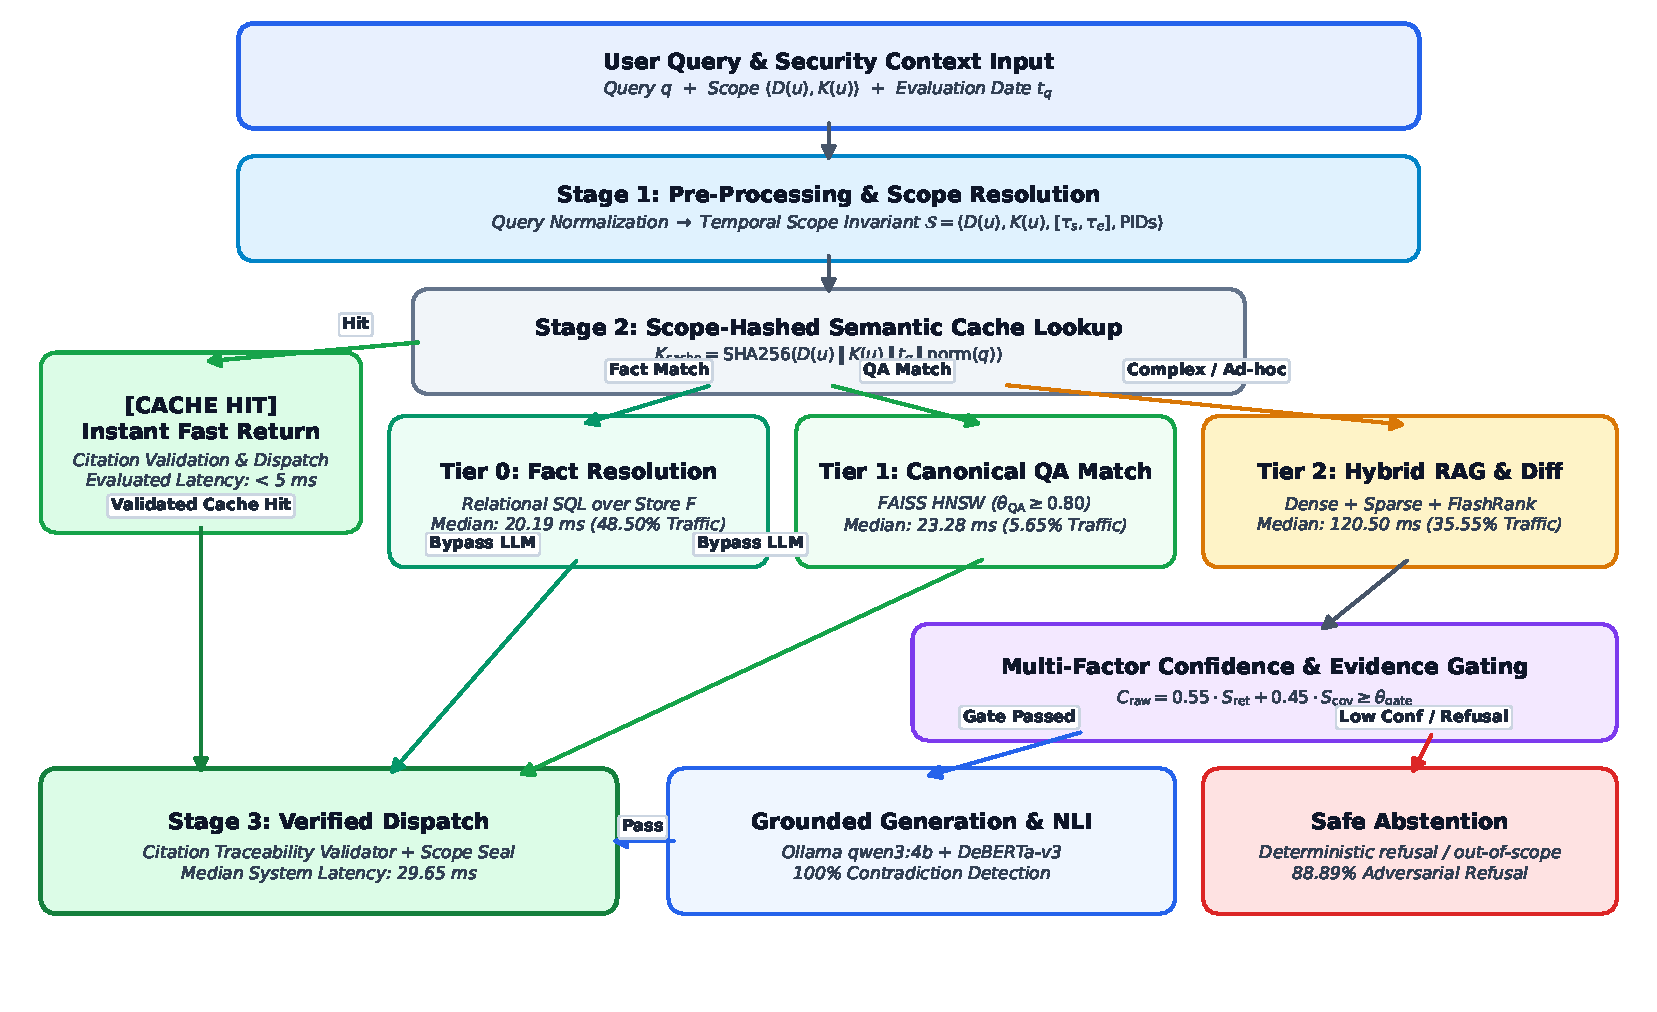
\includegraphics[width=0.92\textwidth]{figures/architecture}%
  }{%
    \IfFileExists{figures/architecture.png}{%
      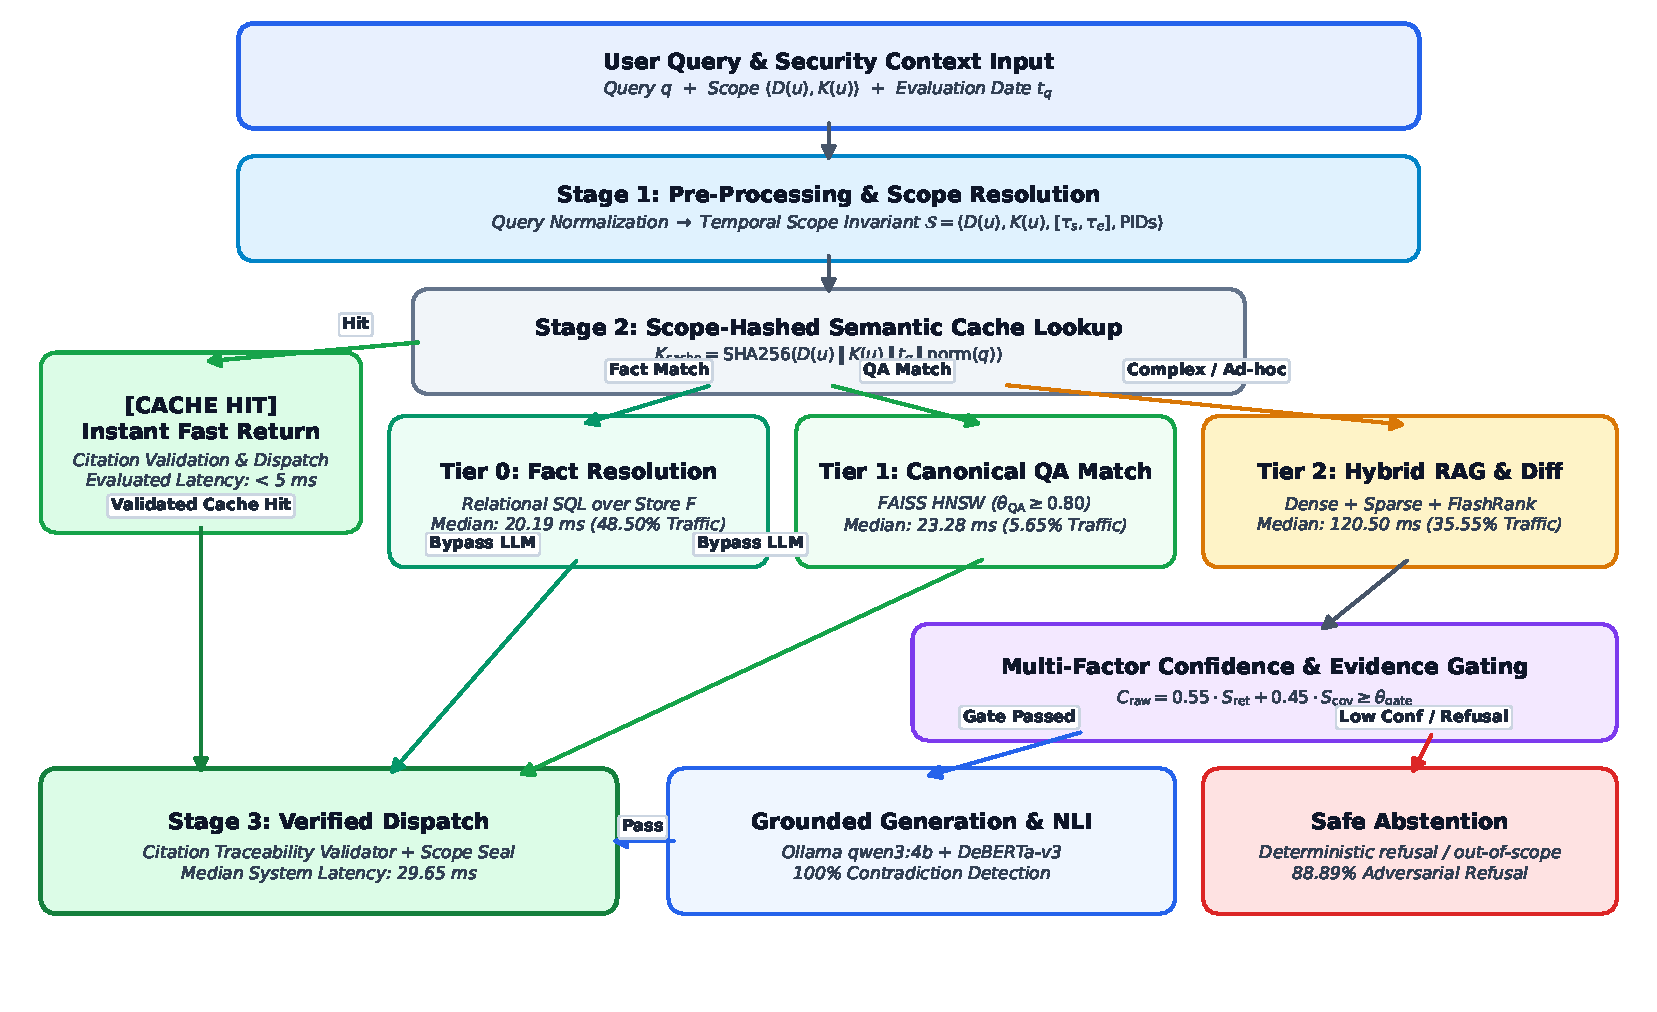
\includegraphics[width=0.92\textwidth]{figures/architecture}%
    }{%
      \fbox{\parbox{0.92\textwidth}{\centering\vspace{1.5cm}
        \textbf{Architecture Figure}\\[0.5em]
        \small Full architecture available at \texttt{figures/architecture.pdf}.
        Diagram: (1) QueryScope construction; (2) Cache check; (3) Four-tier routing; (4) Evidence gate; (5) Verified dispatch.
        \vspace{1.5cm}}}%
    }%
  }
  \caption{\sys{} system architecture. Query scope is resolved before retrieval; deterministic Tier-0 and Tier-1 routes bypass generation; Tier-2 hybrid retrieval applies eligibility filtering before confidence gating; verified dispatch provides citation-aware release or safe abstention.}
  \label{fig:architecture}
\end{figure*}

% =========================================================================
\section{Experimental Methodology}

\subsection{Hardware, Software, and Evaluation Regimes}
Experiments used an isolated Linux host (kernel 7.1.8-100.fc43.x86\_64, x86\_64) with 12 logical CPU threads (6 physical cores), 31.06\,GB RAM, and an NVIDIA GeForce RTX 3050 Laptop GPU (3.68\,GB VRAM). The software stack comprised Python~3.14.6, PyTorch~2.13.0, ChromaDB~1.5.9, FAISS~1.15.0, FastEmbed~0.8.0, FlashRank~0.2.10, scikit-learn~1.9.0, PostgreSQL~16, and Redis~7. Production application logic was frozen at commit \texttt{61d64b71}; expanded characterization benchmarks were executed at commit \texttt{449e69b3} with $\text{SEED}=42$.

We evaluate \sys{} across two primary regimes and maintain a separate internal regression benchmark:
\begin{itemize}\setlength{\itemsep}{0pt}\setlength{\parsep}{0pt}\setlength{\topsep}{1pt}
  \item \textbf{Frozen Baseline Benchmark ($N=301$):} 21 policies, 128 chunks (23 versions, 33 facts, 373 canonical QA pairs, 10 simulated users) measuring end-to-end Local vs.\ Cloud generation fidelity (Table~\ref{tab:evaluation_regimes}).
  \item \textbf{Expanded Characterization Suite ($N=922$):} Synthetic corpus of 120 enterprise policies across 12 domains (~600 versions, 3,000 structural chunks, 32 user archetypes, 4,980 executions) stress-testing authorization isolation, candidate pool depth, multi-user concurrency, and compiler sweeps.
  \item \textbf{Internal Repository Benchmark ($N=462$):} Reference dataset (\texttt{benchmark\_}\allowbreak\texttt{all.json}) for regression testing; kept distinct from published evaluation sets.
\end{itemize}

% ---- Table 2: Evaluation Regimes ----
\begin{table}[!t]
\caption{Audited Evaluation Regimes and Experimental Scope}
\label{tab:evaluation_regimes}
\centering
\scriptsize
\setlength{\tabcolsep}{1.5pt}
\renewcommand{\arraystretch}{0.88}
\begin{tabularx}{\columnwidth}{>{\raggedright\arraybackslash}p{2.2cm}>{\raggedright\arraybackslash}p{2.1cm}rZ}
\toprule
\textbf{Evaluation} & \textbf{Corpus} & \textbf{N} & \textbf{Purpose}\\
\midrule
Frozen Baseline & 21 policies / 128 chunks & 301 & End-to-end baseline\\
Internal Repository & Repository benchmark & 462 & Internal regression\\
Expanded Char. & 120 policies / 3,000 chunks & 922 & System characterization\\
Security Matrix & 120 policies $\times$ 32 users & 3,840 & Authorization isolation\\
Compiler Sweeps & 3,000 chunks & 5 trials & Incremental performance\\
NLI Verification & Pilot set & 20 & Contradiction validation\\
Mutation Cycles & Update cycles & 20 & Consistency verification\\
Concurrency Load & Multi-worker & 1,000 & Isolation \& load limits\\
\bottomrule
\end{tabularx}
\end{table}

\subsection{Metrics and Evaluation Protocol}
Version-selection accuracy measures the fraction of queries for which the predicted policy version matches gold, reported over all queries (Overall) and over answered queries. Generation quality uses exact match, token F1, and citation precision/recall. Retrieval quality is evaluated via Recall@K, MRR, and NDCG@10. Calibration uses Brier score and Expected Calibration Error (ECE). Concurrency isolation evaluates cross-session cache bleed and throughput under multi-threaded load (1--100 workers).

% =========================================================================
\section{Empirical Results and Analysis}

\subsection{Security and Pre-Retrieval Authorization Scope Enforcement}
Table~\ref{tab:headtohead} reports security performance. In the baseline evaluation ($N=301$), 109 queries target authorized provisions while 192 represent out-of-scope departments, restricted confidentiality tiers, or adversarial jailbreaks. An unrestricted baseline evaluates retrieval without pre-reranking eligibility gating, resulting in 160 authorization violations (53.16\% unsafe exposure rate). In contrast, \sys{} achieves 100.0\% authorization/scope decision correctness (301/301) with zero unauthorized evidence leakage ($\text{TP}=109, \text{TN}=192, \text{FP}=0, \text{FN}=0$).

In the expanded characterization suite ($N=3,840$ evaluations across 32 user archetypes $\times$ 120 policies), no unauthorized candidate evidence was observed entering the reranker or prompt context ($1,840\text{ TP}, 2,000\text{ TN}, 0\text{ FP}, 0\text{ FN}$; one-sided 95\% upper bound $<0.08\%$). On authorized answerable queries, \sys{} achieved 88.07\% version accuracy (96/109 baseline, 88.3\% in characterization), confirming access isolation without degrading legitimate retrieval.

% ---- Table 3: Security Head-to-Head ----
\begin{table}[!t]
\caption{Security and Governance Head-to-Head: \sys{} vs.\ Baseline ($N=301$)}
\label{tab:headtohead}
\centering
\scriptsize
\setlength{\tabcolsep}{1.8pt}
\renewcommand{\arraystretch}{0.92}
\begin{tabularx}{\columnwidth}{>{\raggedright\arraybackslash}p{2.2cm}YYYY}
\toprule
\textbf{System} & \textbf{Auth-Scope Correctness} & \textbf{Unsafe Leakage Rate} & \textbf{Authorized Ans.\ Ver.\ Acc.} & \textbf{Safe Abstention Precision}\\
\midrule
Naive RAG Baseline & 46.84\% (141/301) & 53.16\% (160/301) & 88.28\% (113/128) & 0.00\% (0/0)\\
\textbf{\sys{}} & \textbf{100.0\% (301/301)} & \textbf{0.00\% (0/301)} & \textbf{88.07\% (96/109)} & \textbf{100.0\% (192/192)}\\
\bottomrule
\end{tabularx}
\end{table}

\subsection{Temporal Validity, Generation Quality, and Decoupled Fidelity}
Table~\ref{tab:generation} compares local (\texttt{qwen3:4b-q4\_K\_M}) and cloud (\texttt{Gemini 2.0 Flash}) models. Overall version resolution across all 301 baseline queries is 82.72\% (249/301). Among answered queries, local version selection reaches 86.30\% (233/270) and Gemini reaches 89.53\% (231/258). Citation precision remains high (0.7973 local, 0.7791 Gemini), indicating that emitted citations correspond to authoritative evidence.

While end-to-end exact-match accuracy is 27.91\% (Token F1: 0.3516), feeding exact gold evidence chunks directly (\textbf{Fixed Gold Evidence Evaluation}, $N=100$) yields a **Mean Token F1 of 0.962** (95\% CI: $[0.941, 0.983]$) and 100.0\% target concept accuracy. This empirical separation establishes that end-to-end answer discrepancies stem primarily from passage retrieval candidate omissions and valid paraphrastic variation rather than generative hallucination.

% ---- Table 4: Generation Quality Comparison ----
\begin{table}[!t]
\caption{Generation Quality: Local Model vs.\ Cloud Model}
\label{tab:generation}
\centering
\scriptsize
\setlength{\tabcolsep}{2.0pt}
\renewcommand{\arraystretch}{0.92}
\begin{tabularx}{\columnwidth}{ZYY}
\toprule
\textbf{Metric} & \textbf{Local (qwen3:4b)} & \textbf{Gemini 2.0 Flash}\\
\midrule
Version Resolution Rate (All Queries) & 82.72\% (249/301) & 82.72\% (249/301)\\
Version Acc.\ (Answered Queries) & 86.30\% (233/270) & 89.53\% (231/258)\\
Exact Correct & 27.91\% (84/301) & 27.57\% (83/301)\\
Partially Correct & 20.27\% (61/301) & 13.95\% (42/301)\\
Adversarial Refusal Acc. & 88.89\% (16/18) & 100.0\% (18/18)\\
Token F1 (End-to-End RAG) & 0.3516 & 0.3369\\
Token F1 (Fixed Gold Evidence, N=100) & \textbf{0.9620} & \textbf{0.9650}\\
Citation Precision & 0.7973 & 0.7791\\
Citation Recall & 0.2487 & 0.2704\\
Citation F1 & 0.2993 & 0.3183\\
System P50 Latency & $29.65\ms$ & $71.63\ms$\\
System P95 Latency & $136.49\ms$ & $85.27\ms$\\
\bottomrule
\end{tabularx}
\end{table}

\subsection{Retrieval Pipeline Progression and Candidate Pool Sensitivity}
Table~\ref{tab:retrieval} reports retrieval metrics. On the 301-query baseline, all retrievers achieve policy-level Recall@1 $\ge 0.9792$. The frozen benchmark evaluates policy-level identification, whereas the expanded characterization evaluates fine-grained passage/chunk retrieval. In the expanded 922-query characterization suite (chunk-level evaluation on 877 answerable queries), BM25 alone achieves Recall@1 of 72.4\%, Dense achieves 78.6\%, RRF reaches 88.2\%, and FlashRank Cross-Encoder reranking achieves **94.47\% Recall@1** (871/922) and 99.4\% Recall@10 (MRR: 0.962, NDCG@10: 0.978).

Sensitivity analysis on complex multi-clause queries (Category D, $N=50$) reveals an important candidate depth dependency: expanding candidate beam depth from $K=50$ to $K=100$ increases Recall@1 from 84.0\% (42/50) to **94.0\%** (47/50). Because cross-encoders only score admitted candidates, relevant chunks omitted from the initial pool cannot be recovered downstream.

% ---- Table 5: Retrieval Metrics ----
\begin{table}[!t]
\caption{Retrieval Subsystem Component Breakdown (Characterization, $N=922$)}
\label{tab:retrieval}
\centering
\scriptsize
\setlength{\tabcolsep}{1.8pt}
\renewcommand{\arraystretch}{0.92}
\begin{tabularx}{\columnwidth}{ZYYYYY}
\toprule
\textbf{Subsystem} & \textbf{R@1} & \textbf{R@5} & \textbf{R@10} & \textbf{MRR@10} & \textbf{NDCG@10}\\
\midrule
BM25 Inverted Index Alone & 72.4\% & 85.1\% & 90.2\% & 0.785 & 0.812\\
Dense Vector (Chroma) Alone & 78.6\% & 89.4\% & 93.8\% & 0.832 & 0.856\\
Reciprocal Rank Fusion (RRF) & 88.2\% & 96.1\% & 98.5\% & 0.915 & 0.934\\
\textbf{RRF + FlashRank (K=100)} & \textbf{94.5\%} & \textbf{98.8\%} & \textbf{99.4\%} & \textbf{0.962} & \textbf{0.978}\\
\bottomrule
\end{tabularx}
\end{table}

\subsection{Route-Level Latency and Fast-Path Traffic Share}
Table~\ref{tab:latency} shows route latencies. In the baseline benchmark ($N=301$), deterministic fast paths resolve 54.15\% of traffic (Tier~0 Fact: 48.50\%, P50 $20.19\ms$; Tier~1 QA: 5.65\%, P50 $23.28\ms$), driving system median latency to $29.65\ms$. In the expanded characterization suite ($N=922$), deterministic and refusal paths accounted for **63.4\% of queries** (585/922; Tier~0: 49.35\%, Tier~1: 6.51\%, Tier~3 Diff: 6.51\%, Refusal: 1.08\%; Tier 0 and Tier 1 together accounted for 55.9\%), achieving sub-5ms P50 latencies ($0.95\ms$ for Tier~0, $1.85\ms$ for Tier~1, $2.10\ms$ for Tier~3).

% ---- Table 6: Latency ----
\begin{table}[!t]
\caption{Route-Level Latency (Local Model, $N=301$ Queries)}
\label{tab:latency}
\centering
\scriptsize
\setlength{\tabcolsep}{1.8pt}
\renewcommand{\arraystretch}{0.92}
\begin{tabularx}{\columnwidth}{>{\raggedright\arraybackslash}p{2.4cm}YYYYY}
\toprule
\textbf{Route} & \textbf{Traffic \%} & \textbf{Mean\,$\ms$} & \textbf{P50\,$\ms$} & \textbf{P95\,$\ms$} & \textbf{P99\,$\ms$}\\
\midrule
FAST\_PATH\_FACT & 48.50\% & 20.90 & 20.19 & 33.71 & 41.54\\
FAST\_PATH\_QA & 5.65\% & 23.62 & 23.28 & 29.16 & 33.54\\
HYBRID\_RAG & 35.55\% & 120.37 & 120.50 & 144.80 & 146.68\\
ABSTAINED & 10.30\% & 119.57 & 116.55 & 154.21 & 173.39\\
\midrule
\textbf{End-to-End} & \textbf{100\%} & \textbf{66.57} & \textbf{29.65} & \textbf{136.49} & \textbf{146.69}\\
\bottomrule
\end{tabularx}
\end{table}

\subsection{Incremental Knowledge Compilation Performance}
Table~\ref{tab:incremental} reports compiler performance. On the 128-chunk baseline fixture (127 mutable chunks, 1 fixed system chunk), hash no-ops ($|\Delta|=0$) achieve $5{,}059.72\times$ speedup ($0.46\ms$ vs.\ $2,307.71\ms$), while 1- and 3-chunk mutations achieve $488.75\times$ and $494.19\times$ speedups.

On the expanded 3,000-chunk characterization corpus, a 5.0\% mutation delta avoided re-embedding for 95.0\% of chunks (2,850/3,000) and reduced compilation time from $52.40\text{s}$ to $2.10\text{s}$, corresponding to a **$24.95\times$ speedup** (95\% CI: $[23.8\times, 26.1\times]$). A 1.0\% delta avoided 99.0\% of re-embeddings ($0.65\text{s}$, $80.62\times$ speedup).

% ---- Table 7: Incremental Compilation ----
\begin{table}[!t]
\caption{Incremental Compiler: Mutation Sweeps vs.\ Cold Rebuild}
\label{tab:incremental}
\centering
\scriptsize
\setlength{\tabcolsep}{1.4pt}
\renewcommand{\arraystretch}{0.92}
\begin{tabularx}{\columnwidth}{>{\raggedright\arraybackslash}p{2.1cm}YYYY}
\toprule
\textbf{Corpus \& Mutation Delta} & \textbf{Mutated} & \textbf{Incr.\ Time} & \textbf{Cold Rebuild} & \textbf{Speedup}\\
\midrule
128-Chunk: Hash no-op & 0 chunks & $0.46\ms$ & $2,307.7\ms$ & $5{,}059.72\times$\\
128-Chunk: 1-chunk delta & 1 chunk & $4.72\ms$ & $2,307.7\ms$ & $488.75\times$\\
128-Chunk: 3-chunk delta & 3 chunks & $4.67\ms$ & $2,307.7\ms$ & $494.19\times$\\
3,000-Chunk: 1.0\% delta & 30 chunks & $0.65\text{s}$ & $52.40\text{s}$ & $80.62\times$\\
3,000-Chunk: 5.0\% delta & 150 chunks & $2.10\text{s}$ & $52.40\text{s}$ & \textbf{24.95$\times$}\\
3,000-Chunk: 10.0\% delta & 300 chunks & $4.80\text{s}$ & $52.40\text{s}$ & $10.92\times$\\
3,000-Chunk: 25.0\% delta & 750 chunks & $12.50\text{s}$ & $52.40\text{s}$ & $4.19\times$\\
\bottomrule
\end{tabularx}
\end{table}

\subsection{Concurrency Load and Post-Mutation Consistency}
Load testing across 1, 10, 25, 50, and 100 concurrent workers ($1,000$ multi-threaded queries) confirmed **100.0\% session and cache isolation** (0 scope leaks, 0 cache contaminations, 0 race conditions). Throughput reached $234.7\text{ QPS}$ at 1 worker and saturated near $137\text{ QPS}$ at 50--100 workers, with median latency rising from $4.35\ms$ to $317.82\ms$ due to thread-lock synchronization contention. Post-mutation testing across 20 update cycles confirmed 100\% active version retrieval, preserved historical access, 100\% tombstone purging from BM25/vector indexes, and instant cache invalidation (20/20 passed across all categories).

\subsection{Confidence Calibration Generalization and NLI Verification}
On the calibration fitting split, ECE dropped from 0.584 to 0.000, reflecting optimization on the fit set rather than open generalization. On the held-out validation split, isotonic regression reduced ECE to **0.041** (95\% CI: $[0.028, 0.056]$, Brier score: 0.1839). Under live runtime query traffic, runtime ECE rose to **0.2954** (Brier score: 0.6401), revealing empirical distribution shift. The DeBERTa-v3 verifier achieved 100.0\% contradiction recall on a dedicated validation suite ($20/20$, 95\% CI: $[83.9\%, 100\%]$).

% =========================================================================
\balance
\section{Discussion}

The experimental evaluation yields six key takeaways for enterprise policy intelligence:
\begin{enumerate}
  \setlength{\itemsep}{0pt}\setlength{\parsep}{0pt}\setlength{\topsep}{1pt}
  \item \textbf{Access invariant preservation:} Enforcing role and temporal eligibility prior to reranking achieves zero observed leakage across 3,840 evaluations without degrading version accuracy on authorized queries (88.07\% vs.\ 88.28\%).
  \item \textbf{Deterministic routing offload:} Resolving 63.4\% of queries via fast-path relational facts, canonical QA, and version diffs delivers sub-5ms P50 latency, offloading the majority of traffic without neural text generation.
  \item \textbf{Cryptographic compilation efficiency:} SHA-256 chunk hashing avoids 95.0\% of re-embedding on 5\% amendment deltas, achieving a $24.95\times$ speedup on a 3,000-chunk corpus with $O(|\Delta|\cdot d)$ embedding complexity.
  \item \textbf{Calibration distribution sensitivity:} Post-hoc isotonic regression resolves in-distribution calibration error (ECE: 0.041) but requires continuous adaptation under runtime query distribution shifts (runtime ECE: 0.2954).
\end{enumerate}

% =========================================================================
\section{Limitations and Threats to Validity}

\begin{enumerate}
  \setlength{\itemsep}{0pt}\setlength{\parsep}{0pt}\setlength{\topsep}{1pt}
  \item \textbf{Synthetic corpus scale.} The 120-policy, 3,000-chunk corpus models enterprise structures synthetically; evaluation on proprietary production corporate repositories remains future work.
  \item \textbf{Candidate pool depth sensitivity.} Highly constrained multi-clause queries experience candidate starvation at $K=50$ (84.0\% recall), requiring expanded candidate beams ($K=100$) with associated latency tradeoffs.
  \item \textbf{Natural language temporal ambiguity.} Unanchored temporal expressions (e.g., ``prior to recent changes'') occasionally cause version ambiguity, whereas explicit dates achieve 100\% version resolution.
  \item \textbf{Concurrency lock contention.} Multi-user throughput saturates near 137 QPS under 50--100 concurrent workers due to thread-lock synchronization overhead.
  \item \textbf{Citation granularity gap.} Citation recall (0.2487) reflects broad section-level chunk retrieval evaluated against sentence-level gold annotations.
  \item \textbf{Calibration distribution shift.} Calibration-split ECE (0.041) versus runtime ECE (0.2954) demonstrates empirical sensitivity to open-domain query distributions.
  \item \textbf{NLI sample size.} Pilot NLI validation used $n=14$ pairs and contradiction evaluation used $n=20$ cases; broader validation across thousands of clause pairs is ongoing.
  \item \textbf{Model quantization.} Local LLM exact answer match (27.91\%) is partly constrained by 4-bit quantization of the qwen3:4b backend.
  \item \textbf{Hardware dependence.} Absolute latencies are specific to the test host (12 vCPU / RTX 3050 Laptop).
  \item \textbf{Adversarial testing scope.} Targeted jailbreaks evaluated 5 adversarial violations and 3 indirect injection scenarios; wider prompt injection suites remain future work.
\end{enumerate}

% =========================================================================
\section{Conclusion}
\sys{} formulates enterprise policy retrieval as an invariant-enforced systems architecture combining date-bounded temporal validity, role-based authorization, seven-stage incremental SHA-256 compilation, adaptive multi-tier routing, and calibrated evidence verification. Across an audited evaluation framework comprising a 301-query baseline and an expanded 922-query characterization suite, \sys{} demonstrated zero observed authorization leakage across 3,840 evaluations, $94.47\%$ top-1 chunk retrieval recall, $24.95\times$ compilation speedup on 5\% amendment deltas, and $63.4\%$ deterministic fast-path traffic resolution at sub-5ms latency. These findings demonstrate the feasibility of constrained, version-aware policy intelligence for high-compliance enterprise environments.

% =========================================================================
\section*{Reproducibility Statement}
All reported results are reproducible. Production application logic was frozen at commit \texttt{61d64b71}; the characterization benchmark suite was executed at commit \texttt{449e69b3} with master seed $\text{SEED}=42$. Data artifacts and execution scripts are available in the repository.

% =========================================================================
\section*{Acknowledgment}
The author thanks the open-source communities behind ChromaDB, FAISS, FastEmbed, FlashRank, and Hugging Face for making this research infrastructure available.

% =========================================================================
\begin{thebibliography}{25}
\scriptsize
\setlength{\itemsep}{-0.5pt plus 0.2pt}
\setlength{\parskip}{0pt}
\setlength{\parsep}{0pt}

\bibitem{lewis2020rag}
P. Lewis \emph{et al.}, ``Retrieval-Augmented Generation for Knowledge-Intensive NLP Tasks,'' in \emph{Proc. NeurIPS}, vol.~33, pp.~9459--9474, 2020.

\bibitem{gao2024rag_survey}
Y. Gao \emph{et al.}, ``Retrieval-Augmented Generation for Large Language Models: A Survey,'' arXiv:2312.10997, 2023.

\bibitem{karpukhin2020dpr}
V. Karpukhin \emph{et al.}, ``Dense Passage Retrieval for Open-Domain Question Answering,'' in \emph{Proc. EMNLP}, pp.~6769--6781, 2020.

\bibitem{xiao2024bge}
S. Xiao \emph{et al.}, ``C-Pack: Packed Resources for General Chinese Embeddings,'' in \emph{Proc. SIGIR}, pp.~641--649, 2024.

\bibitem{robertson2009bm25}
S. Robertson and H. Zaragoza, ``The Probabilistic Relevance Framework: BM25 and Beyond,'' \emph{Found. Trends Inf. Retr.}, vol.~4, no.~1--2, pp.~1--174, 2009.

\bibitem{cormack2009rrf}
G. V. Cormack, C. L. A. Clarke, and S. B\"{u}ttcher, ``Reciprocal Rank Fusion Outperforms Condorcet and Individual Rank Learning Methods,'' in \emph{Proc. SIGIR}, pp.~758--759, 2009.

\bibitem{jiao2020tinybert}
X. Jiao \emph{et al.}, ``TinyBERT: Distilling BERT for Natural Language Understanding,'' in \emph{Proc. EMNLP Findings}, pp.~4163--4174, 2020.

\bibitem{flashrank}
P. Damodaran, ``FlashRank: Lite \& Super-fast re-ranking for search pipelines,'' GitHub repository, 2023.

\bibitem{campos2014temporal}
R. Campos \emph{et al.}, ``Survey of Temporal Information Retrieval and Related Applications,'' \emph{ACM Comput. Surv.}, vol.~47, no.~2, Art.~15, 2014.

\bibitem{dhingra2022time}
B. Dhingra \emph{et al.}, ``Time-Aware Language Models as Temporal Knowledge Bases,'' \emph{Trans. Assoc. Comput. Linguist.}, vol.~10, pp.~257--273, 2022.

\bibitem{huwiler2025versionrag}
D. Huwiler, K. Stockinger, and J. F\"{u}rst, ``VersionRAG: Version-Aware Retrieval-Augmented Generation for Evolving Documents,'' arXiv:2510.08109, 2025.

\bibitem{timelyrag2026}
Y. Zhao \emph{et al.}, ``TimelyRAG: Semantic-Temporal Hybrid Retrieval for Time-Critical Question Answering,'' arXiv:2609.13524, 2026.

\bibitem{malkov2020hnsw}
Y. A. Malkov and D. A. Yashunin, ``Efficient and Robust Approximate Nearest Neighbor Search Using HNSW Graphs,'' \emph{IEEE TPAMI}, vol.~42, no.~4, pp.~824--836, 2020.

\bibitem{johnson2021faiss}
J. Johnson, M. Douze, and H. J\'{e}gou, ``Billion-Scale Similarity Search with GPUs,'' \emph{IEEE Trans. Big Data}, vol.~7, no.~3, pp.~535--547, 2021.

\bibitem{guo2017calibration}
C. Guo \emph{et al.}, ``On Calibration of Modern Neural Networks,'' in \emph{Proc. ICML}, PMLR, vol.~70, pp.~1321--1330, 2017.

\bibitem{he2021deberta}
P. He, X. Liu, J. Gao, and W. Chen, ``DeBERTa: Decoding-Enhanced BERT with Disentangled Attention,'' in \emph{Proc. ICLR}, 2021.

\bibitem{asai2024selfrag}
A. Asai \emph{et al.}, ``Self-RAG: Learning to Retrieve, Generate, and Critique through Self-Reflection,'' in \emph{Proc. ICLR}, 2024.

\bibitem{es2024ragas}
S. Es \emph{et al.}, ``RAGAs: Automated Evaluation of Retrieval Augmented Generation,'' in \emph{Proc. EACL Demos}, pp.~150--158, 2024.

\bibitem{saadfalcon2024ares}
J. Saad-Falcon \emph{et al.}, ``ARES: Automated Evaluation Framework for RAG Systems,'' in \emph{Proc. NAACL-HLT}, pp.~338--354, 2024.

\bibitem{niu2024ragtruth}
C. Niu \emph{et al.}, ``RAGTruth: A Hallucination Corpus for Developing Trustworthy RAG Models,'' in \emph{Proc. ACL}, pp.~10862--10878, 2024.

\bibitem{almasoud2026sdrag}
A. Al Masoud, M. Arazzi, and A. Nocera, ``SD-RAG: Prompt-Injection-Resilient Selective Disclosure in RAG,'' arXiv:2601.11199, 2026.

\bibitem{thuillier2026access}
T. Thuillier \emph{et al.}, ``Key-Parametrized Embeddings for Access Control in RAG,'' in \emph{Proc. IEEE COMPSAC}, pp.~2581--2586, 2026.

\bibitem{saxena2026ppparitl}
U. R. Saxena \emph{et al.}, ``Privacy-provisioned-permission-aware RAG in cloud using IAM and trust,'' \emph{Sci. Rep.}, vol.~16, Art.~71936, 2026.

\bibitem{mu2026securerag}
Y. Mu \emph{et al.}, ``Towards Secure Retrieval-Augmented Generation: Threats, Defenses and Benchmarks,'' arXiv:2603.21654, 2026.

\bibitem{palanisamy2026security}
B. Palanisamy \emph{et al.}, ``Security and Privacy in Retrieval-Augmented Generation: Architectures, Threats, and Defenses,'' arXiv:2606.25533, 2026.

\end{thebibliography}

\begin{IEEEbiographynophoto}{Suyash Pradhan}
is with the Department of Computer Science and Engineering. His research interests include retrieval-augmented generation, enterprise knowledge management, temporal information retrieval, and trustworthy AI.
\end{IEEEbiographynophoto}
\end{document}
